\documentclass[10pt,letterpaper]{article}
%\usepackage{times}
\usepackage[margin=1in,hmargin=1in]{geometry}
\usepackage{amsmath}
\usepackage{tikz,url}
\usepackage{amssymb}
\usepackage{fancyhdr}
\usetikzlibrary{matrix}
\usepackage{listings}
\usepackage{tabularx}
\usepackage{xcolor}
\usepackage{graphicx}
\usepackage{graphics}
\usepackage{titling}
\pagestyle{fancy}
\usepackage{float}
\usepackage{fancyvrb}
\usepackage{verbatim}
\usepackage{enumitem}
\usepackage{alltt}
\usepackage{pdfpages}
%\usepackage{float}
%\restylefloat{table}

\fancyhead[LO]{STAT W4201 Advanced Data Analysis}
\fancyhead[RO]{HW 6}
\fancyhead[LE]{STAT W4201 Advanced Data Analysis}
\fancyhead[RE]{HW 6}
\title{\textbf {Homework 6}}
\author{{Qianbo Wang}\\{uni: qw2180}}
\date{}
\setlength{\droptitle}{-5em}
\setlength{\parindent}{0pt}
\makeatletter
\newcommand{\rmnum}[1]{\romannumeral #1}
\newcommand{\Rmnum}[1]{\expandafter\@slowromancap\romannumeral #1@}
\makeatother
\lstset{
language=R,
tabsize=4, 
%frame=shadowbox, 
commentstyle=\color{red!50!green!50!blue!50},
%rulesepcolor=\color{red!20!green!20!blue!20},
keywordstyle=\color{blue!90},
showstringspaces=false,
stringstyle=\ttfamily, 
keepspaces=true, 
breakindent=22pt, 
numbers=none,
stepnumber=1,
numberstyle=\tiny, 
numberstyle={\color[RGB]{0,192,192}\tiny} ,
numbersep=5pt,  
basicstyle=\footnotesize, 
showspaces=false, 
flexiblecolumns=true, 
comment=[l]{\#},
texcl=true,
escapeinside={\$$}{\^^M},
breaklines=true, 
breakautoindent=true,
breakindent=4em, 
aboveskip=1em, 
tabsize=2,
showstringspaces=false, 
backgroundcolor=\color[RGB]{244,244,244},   
fontadjust,
captionpos=t,
framextopmargin=2pt,framexbottommargin=2pt,abovecaptionskip=-3pt,belowcaptionskip=3pt,
extendedchars=false,columns=flexible
}

\begin{document}

\maketitle
\thispagestyle{fancy}
\vspace{-2em}

{\large{\textbf{Consider the ChickWeight data in R. The body weights of the chicks were measured at birth (i.e., time=0) and every second day thereafter until day 20. They were also measured on day 21. There were four groups of chicks on different protein diets.}}}

\section*{Problem 1}
\textbf{Determine whether there is a significant difference in the mean weights of the four groups on Day 18.}
\begin{enumerate}[leftmargin=0cm,itemindent=.5cm,labelwidth=\itemindent,labelsep=0cm,align=left]
\item[\textbullet] \textbf{Without adjusting for Birth Weight.}

Since without adjusting for Birth Weight, the model is just simple one-way anova. The anova table is as follows:
\begin{center}
Anova without adjusting for Birth Weight
\verbatiminput{anova.txt}
\end{center} 
Since for F-test, the null and alternative hypothesis are:
\[H_0: \mu_1=\mu_2=\mu_3=\mu_4\]
\[H_1: \mu_i \neq \mu_j  \ \text{for at least one pair (i , j)},\  i \neq j\]
And the $p-value = 0.0072<0.05$. Then we should reject the null hypothesis, i.e. there is a significant difference in the mean weights of the four groups on Day 18. 

\item[\textbullet] \textbf{Adjusting for Birth Weight. Give the LS Means (i.e., adjusted for Birth Weight).}

Since we need do anova analysis based on adjusting for Birth Weight, then we simply add a new variable as Birth Weight, i.e. Give the LS means. Then this time the model is anovca. The anovca table is as follows:
\begin{center}
Anova with adjusting for Birth Weight
\verbatiminput{anova_adjust.txt}
\end{center} 

And the Birth Weight means of the four groups is as follows:
\begin{table}[h]
\caption{Birth Weight LS Means}
\centering
\begin{tabular*}{0.5\linewidth}{@{\extracolsep{\fill}}ccc}
\hline 
Diet & Birth Weight mean & LS mean\\
\hline
1 & 41.58824 & 164.2240\\
\hline
2 & 40.70000 & 183.2445\\
\hline
3 & 40.70000 & 229.7409\\
\hline
4 & 41.00000 & 201.7337\\
\hline
\end{tabular*}
\end{table}
Since this time for F-test, the null and alternative hypothesis are:
\[H_0: \hat{\mu_1}=\hat{\mu_2}=\hat{\mu_3}=\hat{\mu_4}\]
\[H_1: \hat{\mu_i} \neq \hat{\mu_j}  \ \text{for at least one pair (i , j)},\  i \neq j\]
And the $p-value$ for Birth Weight is $p-value = 0.0178<0.05$ and $p-value$ for Diet is $p-value = 0.0234<0.05$. Then we should reject the null hypothesis, i.e. there is a significant difference in the mean weights of the four groups on Day 18 regarding the Birth Weight differences.

\item[\textbullet]\textbf{Check the validity of your assumptions, including parallelism. Suggest measures that you would take if the assumptions are not satisfied.}

Since the assumptions are: \\
\textbullet \ ~i.i.d. normal\\
\textbullet \ ~constant variance
\begin{enumerate}[leftmargin=0cm,itemindent=.5cm,labelwidth=\itemindent,labelsep=0cm,align=left]
\item[\textbf{1.}] \textbf{Check i.i.d. Normality}

First, plot Q-Q plot on residuals, the plot is as follows:
\begin{center}
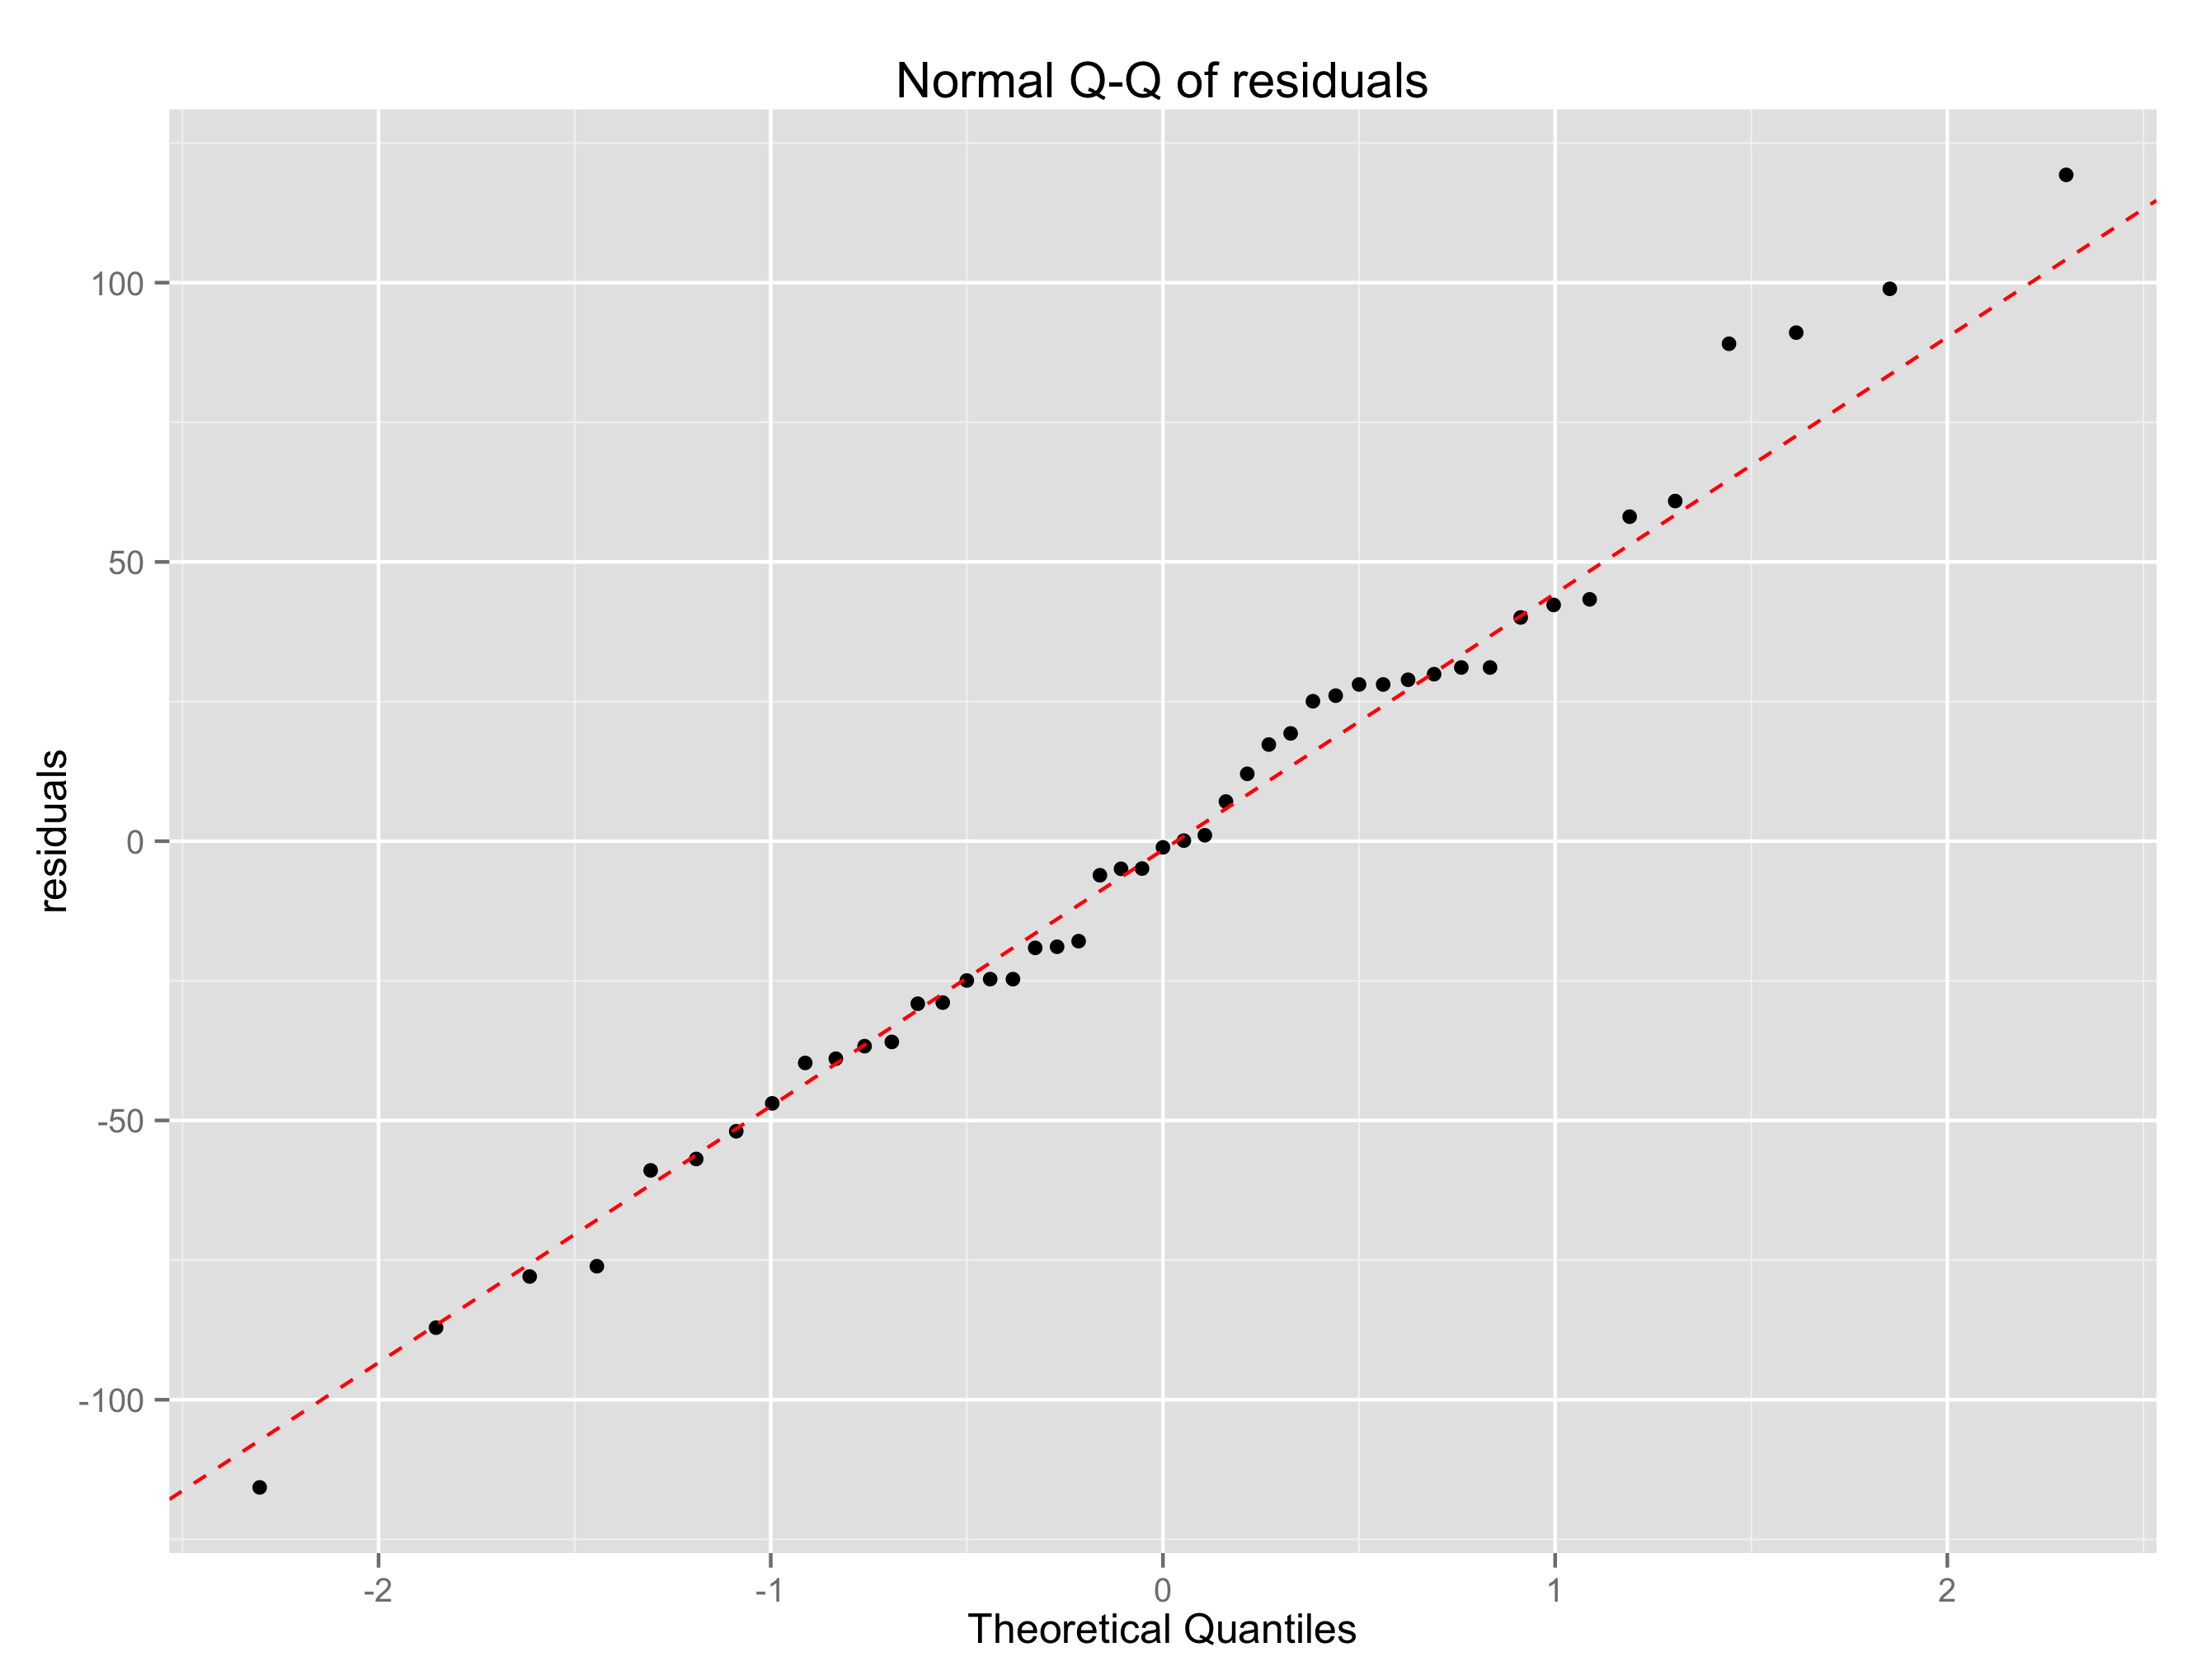
\includegraphics[scale=0.15]{qqplot}
\end{center}
Then, plot histogram with density on residuals, the plot is as follows:
\begin{center}
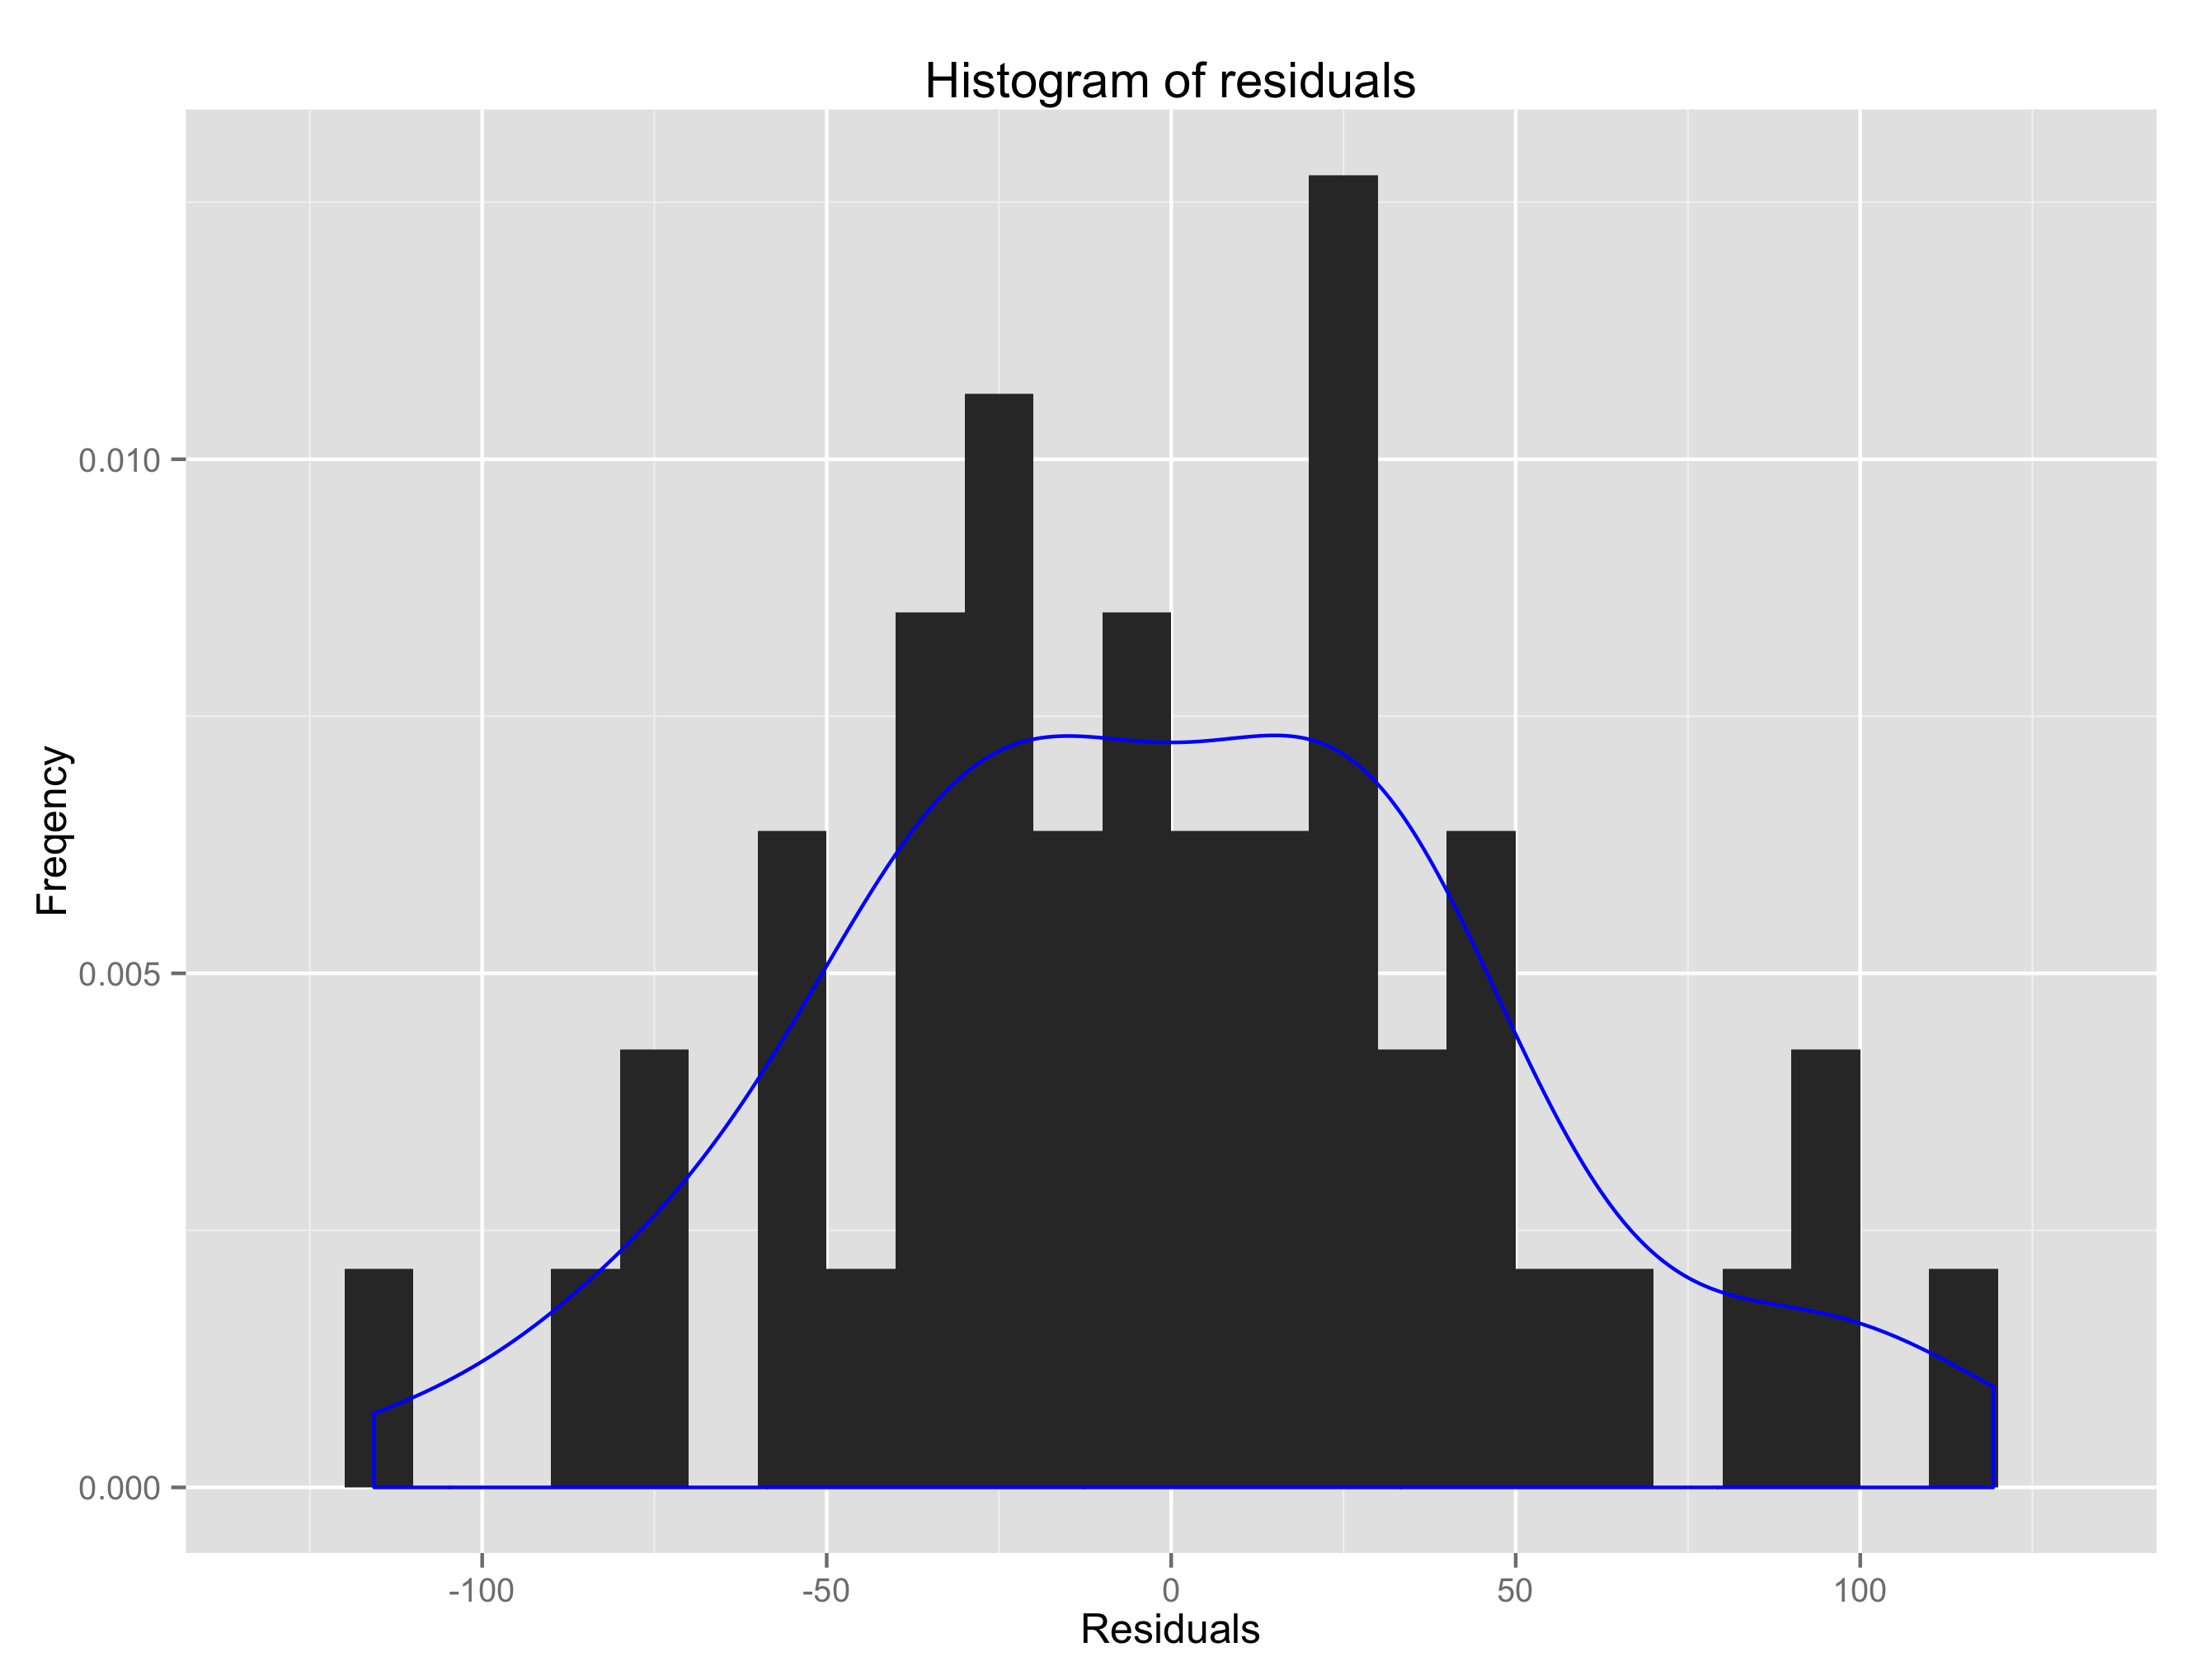
\includegraphics[scale=0.15]{histogram}
\end{center}
Since from the plot, the residuals seem to satisfy normal distribution. Then do Shapiro-Wilk test on residuals, 
The null and alternative hypothesis of Shapiro-Wilk test are:
\[H_0: \epsilon_i \sim \text{Normal}\]
\[H_1: \epsilon_i \ \text{not from Normal}\]

And the Shapiro-Wilk test result is as follows:
\begin{center}
Shapiro-Wilk Test on residuals
\verbatiminput{normalcheck.txt}
\end{center}

Since $p-value = 0.9242$, then we should not reject the null, i.e. the residuals satisfy normal distribution.\\

Then, check the i.i.d. assumption, use nonparametric Kruskal-Wallis test on raw data. The null and alternative hypothesis of Kruskal-Wallis test are:
\[H_0: w_1, w_2, w_3, w_4 \ \text{i.i.d.} \]
\[H_1: w_1, w_2, w_3, w_4\  \text{not i.i.d.} \]
The result is as follows:
\begin{center}
Kruskal-Wallis test on raw data
\verbatiminput{identicalcheck.txt}
\end{center}
Since $p-value=0.01395 $, then we should reject the null, i.e. the weight data in the four Diet group are not from the same distribution. 

\item[\textbf{2.}] \textbf{Check Constant Variance}

First, use Bartlett's on raw data to check the constant variance. The null and alternative hypothesis of  Bartlett's test are:
\[H_0:  {\sigma_1}^2 = ... = {\sigma_4}^2\]
\[H_1:  {\sigma_i}^2 \neq {\sigma_j}^2  \ \text{for at least one pair (i , j)},\  i \neq j\ \]
And the Bartlett's test is highly dependent on the normal assumption, since we have check the validation of normality, then we can use Bartlett's test. The result is as follows:
\begin{center}
Bartlett's test on raw data
\verbatiminput{constantcheck.txt}
\end{center}
Since $p-value=0.3111>0.05$, then we should not reject the null, i.e. the constant variance assumption satisfies.\\

Then use Levene's Test on raw data to check the constant variance. The null and alternative hypothesis of Levene's test are:
\[H_0:  {\sigma_1}^2 = ... = {\sigma_4}^2\]
\[H_1:  {\sigma_i}^2 \neq {\sigma_j}^2  \ \text{for at least one pair (i , j)},\  i \neq j\ \]
The result is as follows:
\begin{center}
Levene's test on raw data
\verbatiminput{levene.txt}
\end{center}
Since $p-value=0.3764>0.05$, then we should not reject the null, i.e. the constant variance assumption satisfies.

\item[\textbf{2.}] \textbf{Check parallelism}

Use two-way anova to check the parallelism,  the null and alternative hypothesis are:
\[H_0: \ \text{there is joint effect with Diet and Birth Weight}\]
\[H_1: \ \text{there is no joint effect with Diet and Birth Weight}\]
The result is as follows:
\begin{center}
Two-way Anova for parallelism check
\verbatiminput{paracheck.txt}
\end{center}
And the $p-value = 0.3530>0.05$. Then we should not reject the null hypothesis, i.e. there is no interaction effect between Diet group and the Birth Weight. So we do not need do marginal inference on BirthWeight and Diet. 
\end{enumerate}
\end{enumerate}

\section*{Problem 2}
\textbf{Perform an appropriate repeated measures ANOVA to determine whether there is a significant difference in the mean weights of the four groups using the measurements on Days 10, 18, and 21.}
\begin{enumerate}[leftmargin=0cm,itemindent=.5cm,labelwidth=\itemindent,labelsep=0cm,align=left]
\item[\textbullet] \textbf{Do the analyses assuming compound symmetry and unstructured covariance structures and compare the results.}
\begin{enumerate}[leftmargin=0cm,itemindent=.5cm,labelwidth=\itemindent,labelsep=0cm,align=left]
\item[\textbf{1.}] \textbf{Compound Symmetry}

For this part of the problem, I simply use SAS to do the repeat measures ANOVA because SAS has a easily-used implementation of repeated measures ANOVA based on different structure assumptions on covariance.
Since for the assumption, it assumes that the covariance between the data is compound symmetry or unstructured. Then the result is in the following page.
\item[\textbf{2.}] \textbf{Unstructured Covariance}

Since the assumption is unstructured covariance, then the result is in the following page.
\begin{center}
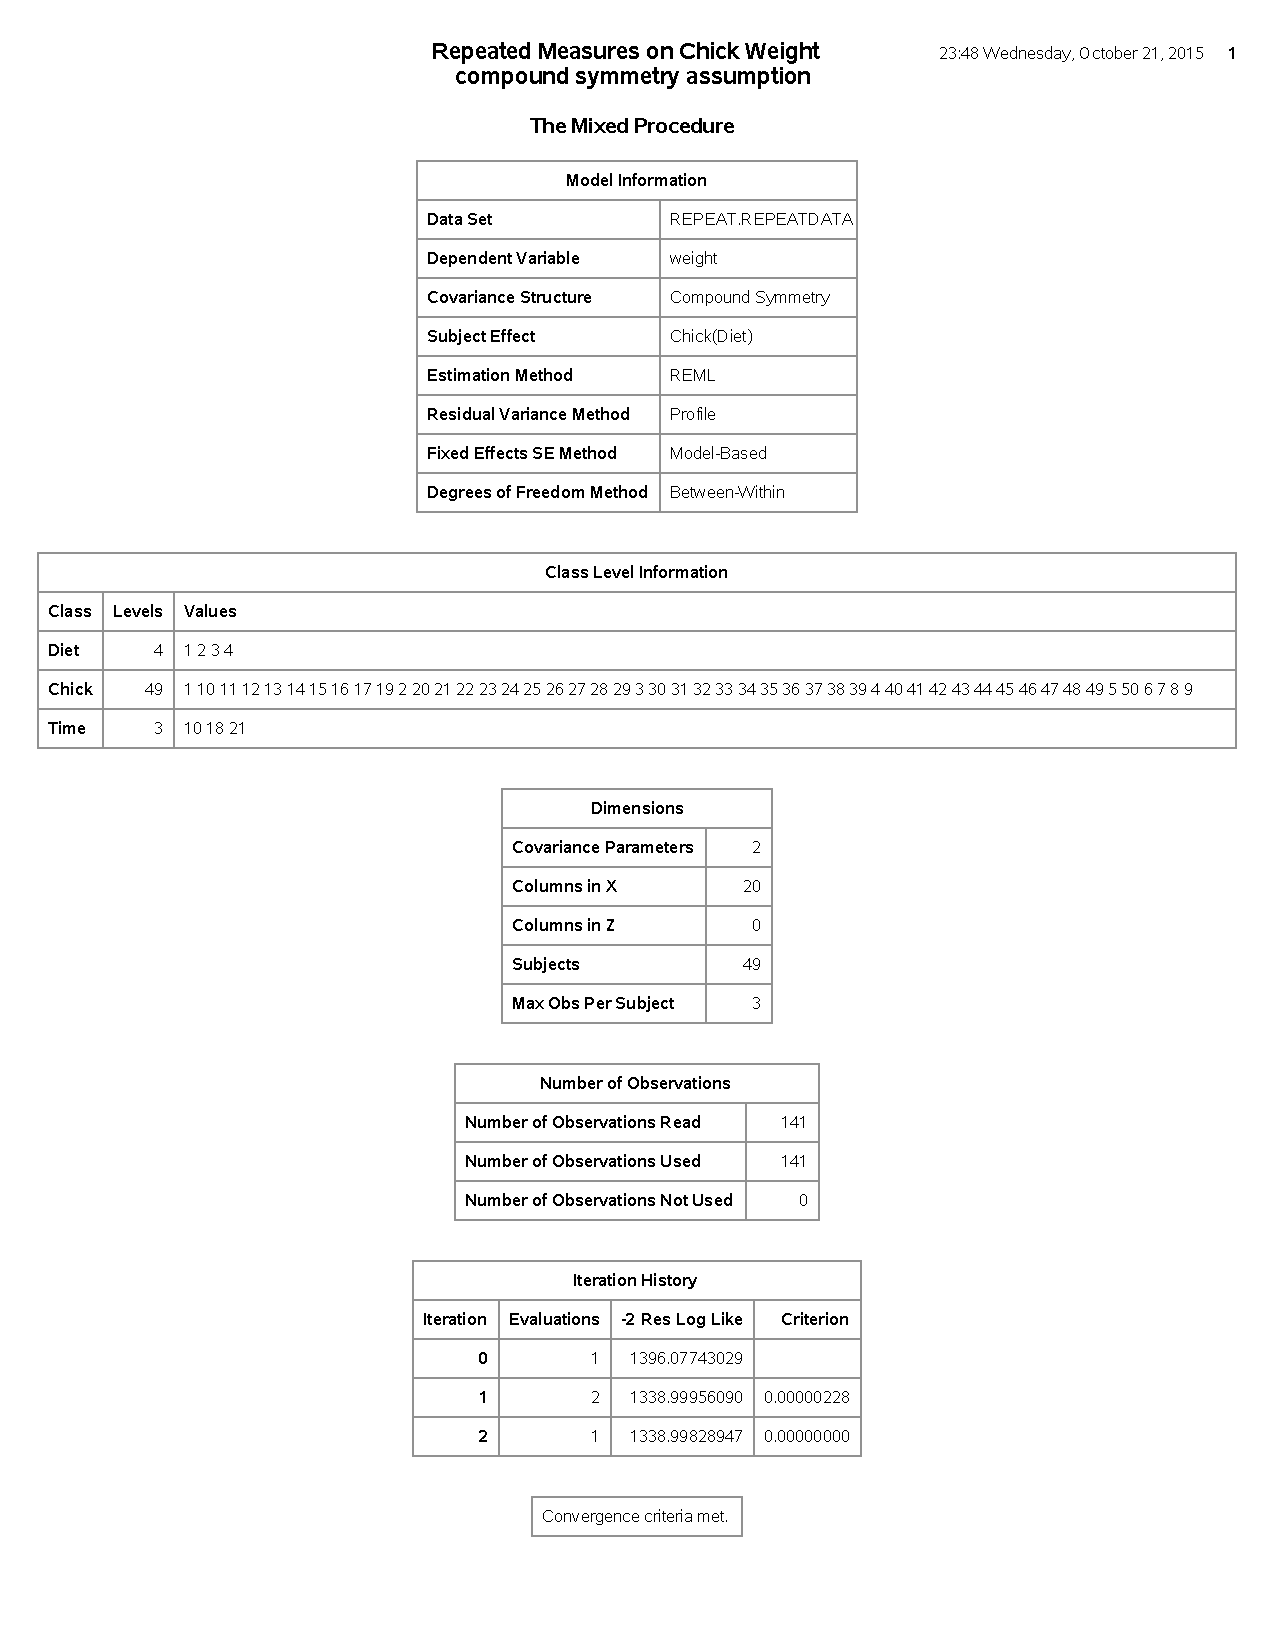
\includepdf[pagecommand={},scale=0.8,pages={1,2}]{compoundsy.pdf}
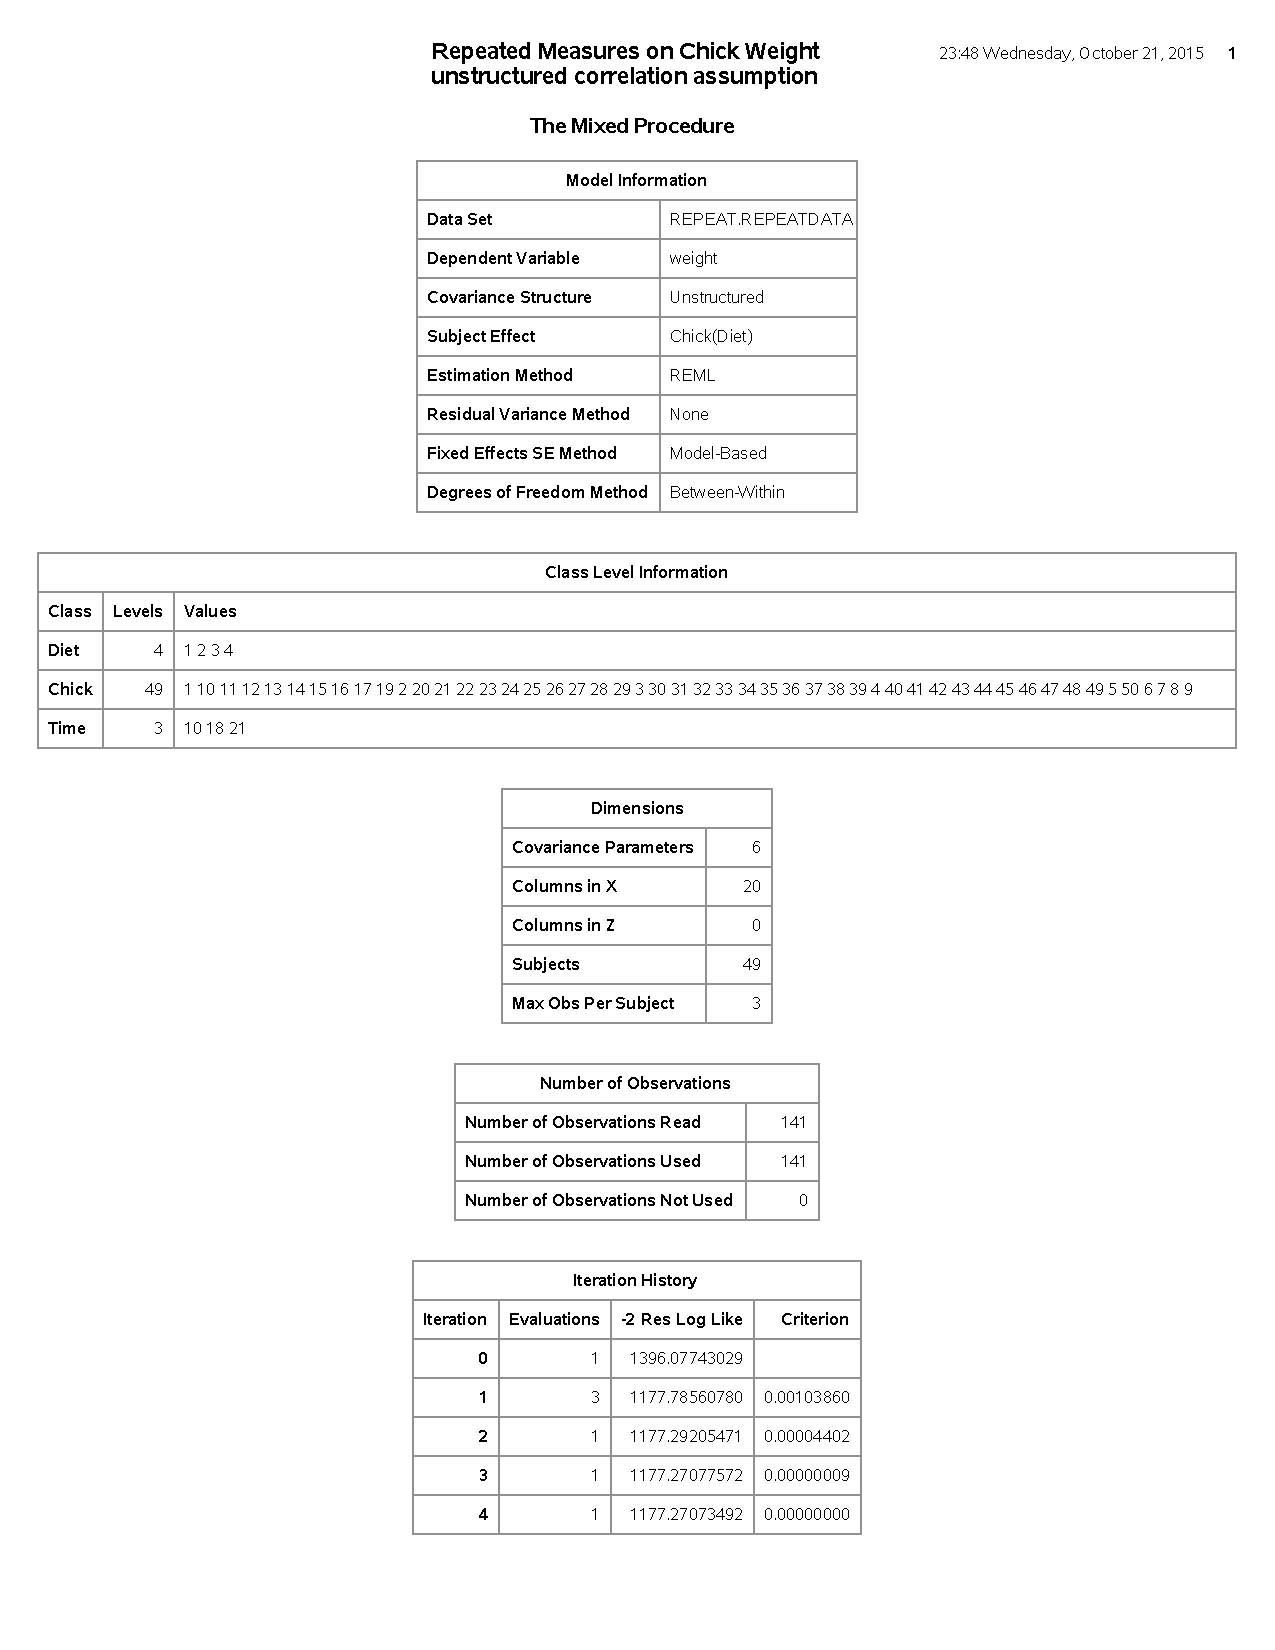
\includepdf[pagecommand={},scale=0.8,pages={1,2}]{unstructured.pdf}
\end{center}
\end{enumerate}
Compare the result:\\
Since both under compound symmetry covariance and unstructured covariance assumption, all of the p-values are significant, then we should conclude that the chicken have significant different of weight on at least two Diet group and between Day 10, Day18 and Day 21. And the differences between the two method on this test is just the different estimation on the covariance structure.\\ 

\item[\textbullet] \textbf{Check the validity of your assumptions.}
\begin{enumerate}[leftmargin=0cm,itemindent=.5cm,labelwidth=\itemindent,labelsep=0cm,align=left]
\item[\textbf{1.}] Normality

Since the assumptions for repeated measures are normality and constant variance. Then under the compound symmetry assumption and unstructured covariance assumption, the plots of the residuals given by SAS are as follows:
Since from the plots, we see that the data is approximately normally distributed.
Then do normal test on residuals, the result is also on the following pages.\\
Since under compound symmetry covariance assumption, for Shapiro-Wilk test on residuals gives the $p-value=0.0212<0.05$, then we should not reject the null, i.e. the normality assumption doesn't satisfy, i.e. it is not normal.\\
And under unstructured covariance assumption, for Shapiro-Wilk test on residuals gives the $p-value=0.0119>0.05$, then we should not reject the null, i.e. the normality assumption doesn't satisfy, i.e. it is not normal.
\item[\textbf{2.}] Constant Variance

Since normality assumption satisfies then use Bartlett's test on raw data gives the $p-value=0.0561>0.05$, then we should not reject the null, i.e. the Constant Variance assumption satisfies.\\
\end{enumerate}

\begin{center}
\includepdf[pagecommand={},scale=0.85,pages={3}]{compoundsy.pdf}
\includepdf[pagecommand={},scale=0.85,pages={3}]{unstructured.pdf}
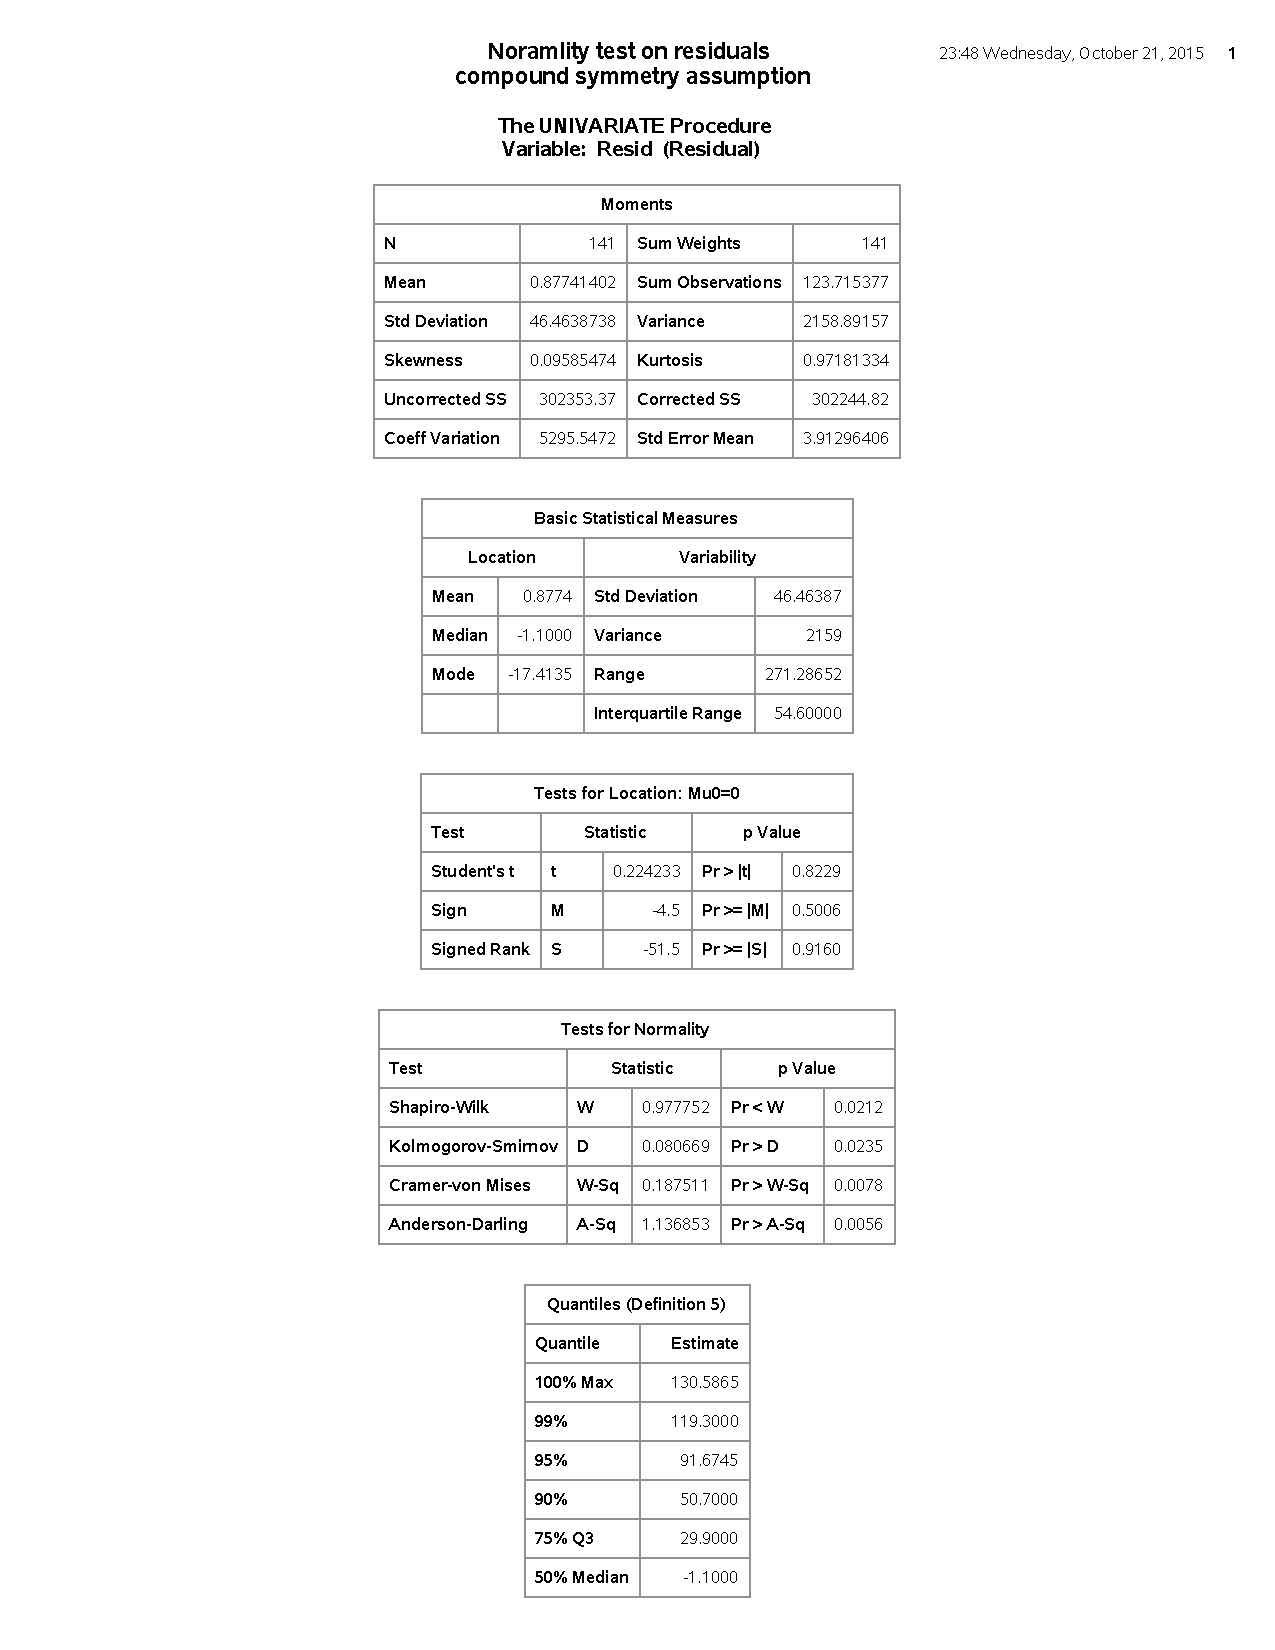
\includepdf[pagecommand={},scale=0.85,pages={1}]{normalcs.pdf}
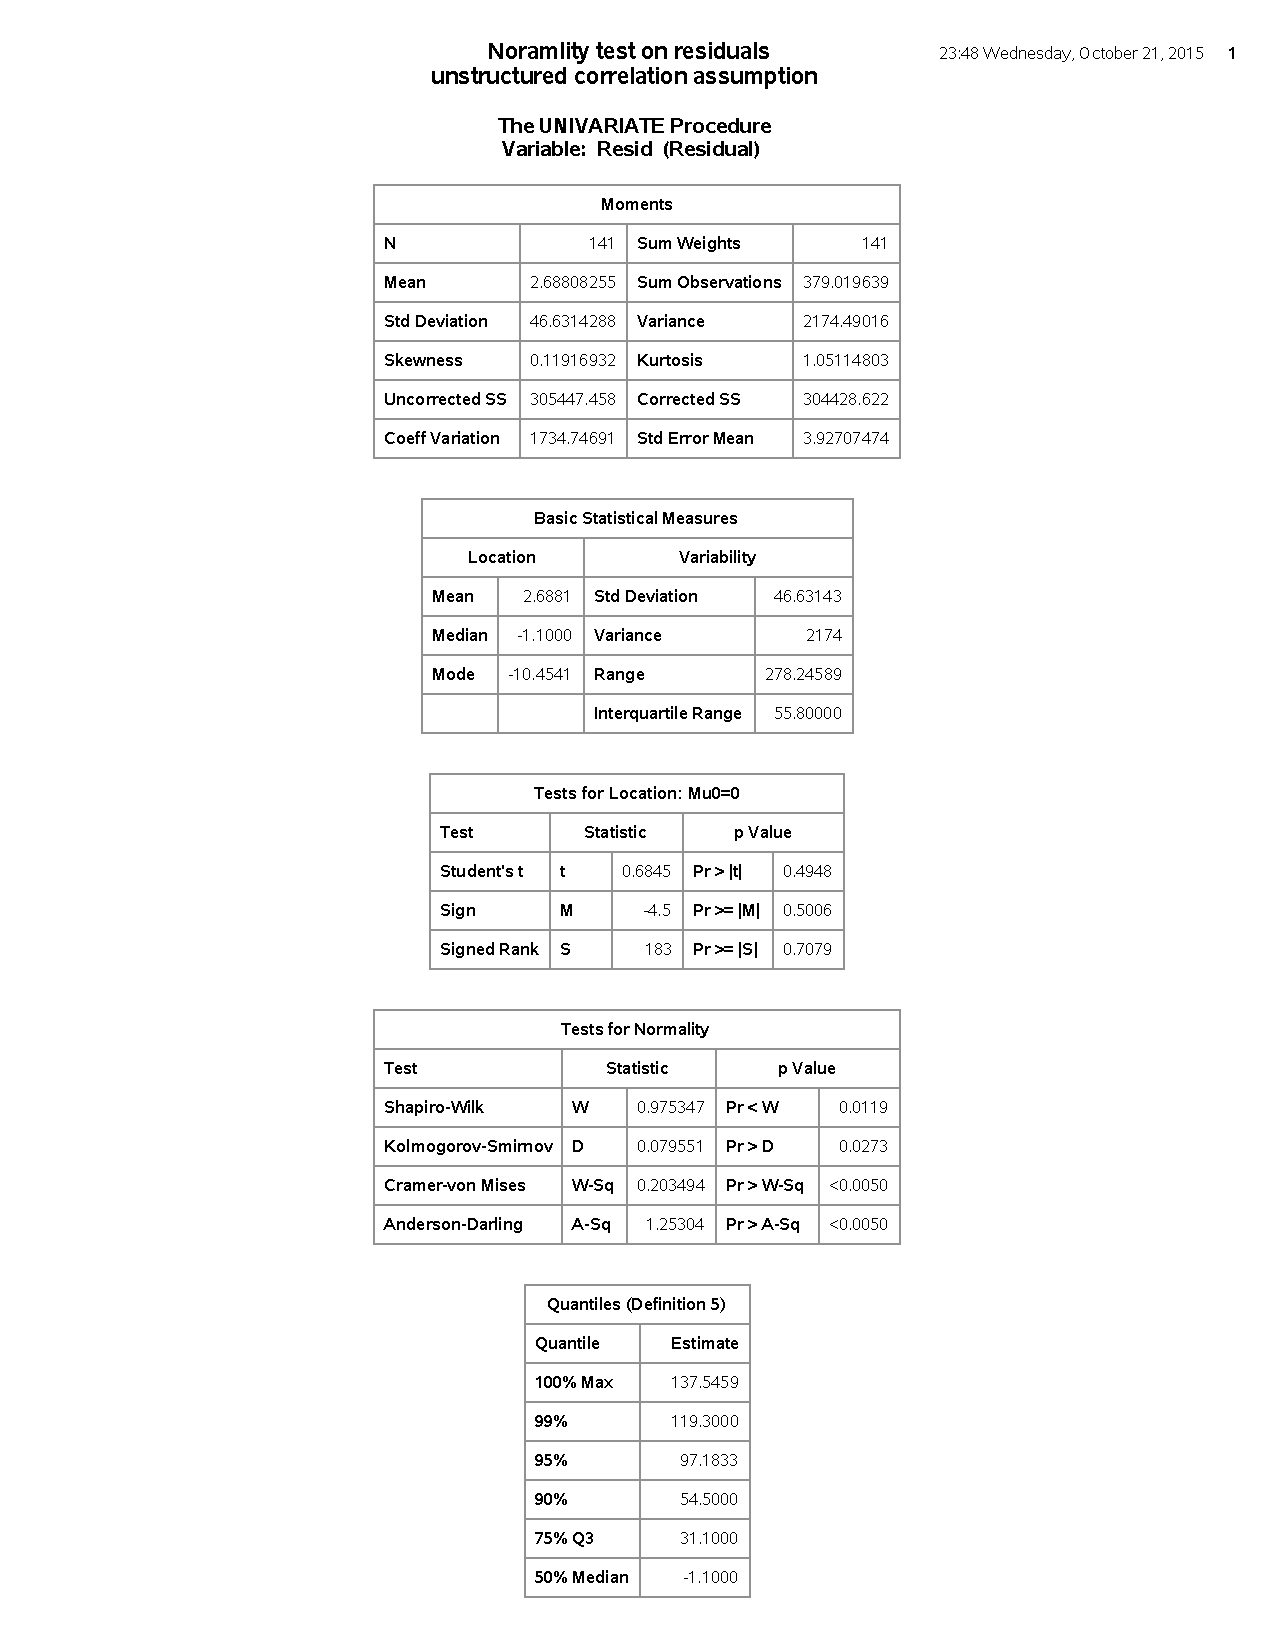
\includepdf[pagecommand={},scale=0.85,pages={1}]{normalun.pdf}
\includepdf[pagecommand={},scale=0.85,pages={3,5}]{homo.pdf}
\end{center}
\end{enumerate}

\newpage
\textbf{R Code:}
\begin{lstlisting}[language=R]
rm(list=ls())
data('ChickWeight')
#avova on day 18
sub_day18<-subset(ChickWeight,Time==18)
anova_day18<-aov(data = sub_day18, weight ~ Diet)
summary(anova_day18)

sink('/Users/raymond/Drive/STAT W4201/HW6/anova.txt')
anova_day18
summary(anova_day18)
sink()

#anova adjust by LS mean on day 18
sub_day0<-subset(ChickWeight,Time==0)
sub_day18[,'birthweight']<-sub_day0$weight[match(sub_day18$Chick,sub_day0$Chick)]
group_mean<-aggregate(sub_day18$birthweight,list(sub_day18$Diet),mean)
colnames(group_mean)<-c('Diet','birthweight_mean')
sub_day18<-merge(sub_day18,group_mean,by.y = 'Diet')
anova_adjust_day18<-aov(data=sub_day18, weight ~ birthweight + Diet)

sink('/Users/raymond/Drive/STAT W4201/HW6/anova_adjust.txt')
anova_adjust_day18
summary(anova_adjust_day18)
sink()

#LS means
coef<-anova_adjust_day18$coefficients[2]
y_hat<-anova_adjust_day18$fitted.values
y_frame<-data.frame(yhat=y_hat,Diet=sub_day18$Diet)
yhat_mean<-aggregate(y_frame$yhat, list(y_frame$Diet),mean)
colnames(yhat_mean)<-c('Diet','yhat')
mu<-yhat_mean$yhat-coef*(group_mean$birthweight_mean-mean(sub_day18$birthweight))
lsmean_result<-cbind(group_mean,lsmean=mu)
sink('/Users/raymond/Drive/STAT W4201/HW6/LSmeans.txt')
lsmean_result
sink()
#Or simply use lsmeans function in library lsmeans
library(lsmeans)
lsmean<-lsmeans(anova_adjust_day18,'Diet')
sink('/Users/raymond/Drive/STAT W4201/HW6/LSmeans1.txt')
lsmean
sink()

library(ggplot2)
#check assumptions
#Normality
#Q-Q plot for residuals
residual<-data.frame(anova_day18['residuals'],sub_day18['Diet'])
normal_plot<-ggplot(data=residual,aes(sample=residuals))+
  stat_qq()+ggtitle('Normal Q-Q of residuals')+
  ylab('residuals')+xlab('Theoretical Quantiles')
resid_quantile<-quantile(residual$residuals,c(0.25, 0.75))
norm_quantile<-qnorm(c(0.25, 0.75))
slope<-diff(resid_quantile)/diff(norm_quantile)
inter<-resid_quantile[1]-slope*norm_quantile[1]
normal_plot+geom_abline(slope=slope,intercept=inter,linetype=2,color='red')
ggsave(filename = '/Users/raymond/Drive/STAT W4201/HW6/qqplot.png')

#histogram for residuals
histogram_plot<-ggplot(data=residual,aes(residuals))+
  geom_bar(binwidth=10,aes(y=..density..))+ggtitle("Histogram of residuals")+
  ylab('Freqency')+xlab('Residuals')
histogram_plot+geom_density(color='blue')
ggsave(filename = '/Users/raymond/Drive/STAT W4201/HW6/histogram.png')

#shapiro test on residuals
shapiro.test(residual$residuals)
sink('/Users/raymond/Drive/STAT W4201/HW6/normalcheck.txt')
shapiro.test(residual$residuals)
sink()

#check constant variance
#bartlett test on data
bartlett.test(x=sub_day18$weight,g=sub_day18$Diet)
sink('/Users/raymond/Drive/STAT W4201/HW6/constantcheck.txt')
bartlett.test(x=sub_day18$weight,g=sub_day18$Diet)
sink()

#levene test on data
library(car)
leveneTest(y=sub_day18$weight,group=as.factor(sub_day18$Diet))

#nonparametric check iid assumptions
#kruskal test on data
kruskal.test(weight~Diet,data=sub_day18)
sink('/Users/raymond/Drive/STAT W4201/HW6/identicalcheck.txt')
kruskal.test(weight~Diet,data=sub_day18)
sink()

#check for parallelism
#two-way anova
anova_inter<-aov(weight ~ birthweight*Diet,data = sub_day18)
summary(anova_inter)
sink('/Users/raymond/Drive/STAT W4201/HW6/paracheck.txt')
summary(anova_inter)
sink()

#repeated measures
#anova on day 10, 18, 21
sub_repeat<-subset(ChickWeight,Time %in% c(10,18,21))
repeated<-aov(weight ~ Diet*Time+Error(Chick),data=sub_repeat)

write.table(sub_repeat,file = '/Users/raymond/Drive/STAT W4201/HW6/ChickWeight.csv',col.names=TRUE,row.names=FALSE,sep=",")
\end{lstlisting}

\newpage
\textbf{SAS code: }
\begin{lstlisting}[language=SAS]
libname repeat 'C:\Users\QIANBO\Desktop\HW6';
*import data from csv;
proc import out=repeat.repeatdata
    Datafile = 'C:\Users\QIANBO\Desktop\HW6\ChickWeight.csv'
    Dbms =csv replace;
run;
proc print data = repeat.repeatdata;
run;

ods listing close;
ods graphics on;
options papersize=letter;
ods pdf file='C:\Users\QIANBO\Desktop\HW6\compoundsy.pdf';
title'Repeated Measures on Chick Weight';
title2'compound symmetry assumption';

*correlation compound symmetry assumption;
proc mixed data = repeat.repeatdata;
class Diet Chick Time;
model weight= Diet Time Diet*Time / outp=repeat.csparam residual;
repeated/type=cs sub=Chick(Diet) rcorr ;
run;
ods pdf close;

ods pdf file='C:\Users\QIANBO\Desktop\HW6\unstructured.pdf';
title'Repeated Measures on Chick Weight';
title2'unstructured correlation assumption';
*correlation unstructured assumption;
proc mixed data = repeat.repeatdata;
class Diet Chick Time;
model weight = Diet Time Diet*Time / outp=repeat.unparam residual;
repeated/type=un sub=Chick(Diet) rcorr;
run;
ods pdf close;
ods graphics off;

ods pdf file='C:\Users\QIANBO\Desktop\HW6\normalcs.pdf';
title'Noramlity test on residuals';
title2'compound symmetry assumption';
*test normality;
proc univariate data=repeat.csparam normal; 
var resid;
run;
ods pdf close;

ods pdf file='C:\Users\QIANBO\Desktop\HW6\normalun.pdf';
title'Noramlity test on residuals';
title2'unstructured correlation assumption';
*test normality;
proc univariate data=repeat.unparam normal; 
var resid;
run;
ods pdf close;

ods pdf file='C:\Users\QIANBO\Desktop\HW6\homo.pdf';
title'Constant Variance test on raw data';
title2;
proc glm data=repeat.repeatdata; 
class Diet Chick Time; 
model weight = Diet;  
means Diet / HOVTEST=BARTLETT;  
means Diet / HOVTEST=LEVENE;
run;
ods pdf close;
ods listing;
title;
\end{lstlisting}
\end{document}